\section{引言}

自主水下航行器（下称航行器）在端侧依据陈旧海流图作航路决策时，必须在继续计算与补充观测之间作出选择。海洋大数据的计算正从岸基中心延伸到移动观测平台，航行器所用的海流信息仍主要来自岸基汇集的卫星与模式产品\cite{chassignet2007hycom,chin2017mur}；然而水下声学通信带宽极窄，上浮通信耗时耗能，机载算力与电池能量也十分有限\cite{remus100,jetsonorinnx}，航行器在长航程任务中所依据的往往是数天前下发的粗分辨率海流图。在台湾以东的黑潮区，长航程航行器约1.0米/秒的对水速度与强流流速相当，绕越禁航区时从左侧还是右侧通行是不可逆的二元决策，选错一侧要多花数小时。图\ref{fig:overview}给出了一个例子：3天前的1°粗分辨率海流图（下称粗图）上左右两侧只差约0.3小时，当天的真实海流中右侧却快11.7小时。此时，航行器应当继续计算，还是去观测？

\begin{figure}[t]
\centering
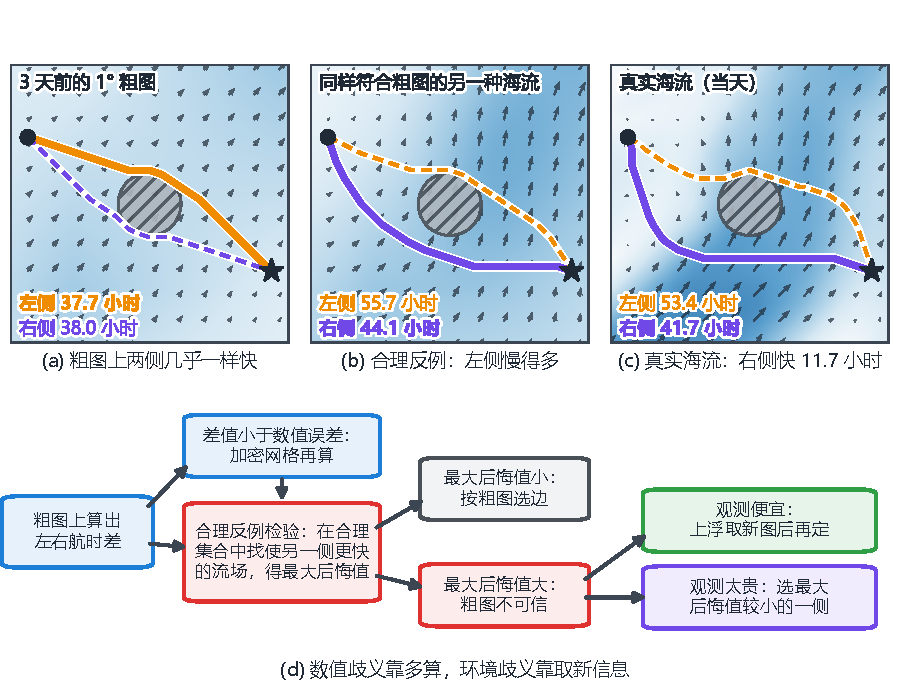
\includegraphics[width=\linewidth]{fig_route_overview}
\caption{粗图下的选边决策与合理反例检验（2022年1月18日测试任务）。(a) 3天前的1°粗图：左侧37.7小时、右侧38.0小时，按粗图选左侧；(b) 合理集合中搜出的合理反例：左侧55.7小时、右侧44.1小时；(c) 当天真实海流：右侧快11.7小时；(d) 本文的决策流程。加算只能把(a)中0.3小时的差值算得更准，合理反例检验则把(b)这样与粗图同样相容、却要求选另一侧的海流显式找出来。}
\label{fig:overview}
\end{figure}

最直接的做法是多算，但当缺失的是环境信息时，多算只会让答案更精细，而不会更正确。加密求解网格、增加航向离散度或增加规划器的推演次数\cite{lolla2014levelset}，只能减小同一张粗图上的离散误差，不能补充粗图缺失的涡旋与切变；规划器在有偏的内部模型上搜索得越久，越会把模型误差当作机会，对自身方案的估值越高\cite{smith2006curse,jiang2015horizon,cuadron2025overthinking}。作者在前期的东海赤潮巡测研究中观察到了这一现象（图\ref{fig:curse}）：航行器携带3天前的卫星叶绿素图，每次决策的推演从64次增至20万次，规划器对自身航线的估值从0.762持续升至0.917，而航线的真实价值约2000次推演后便不再提高。

\begin{figure}[t]
\centering
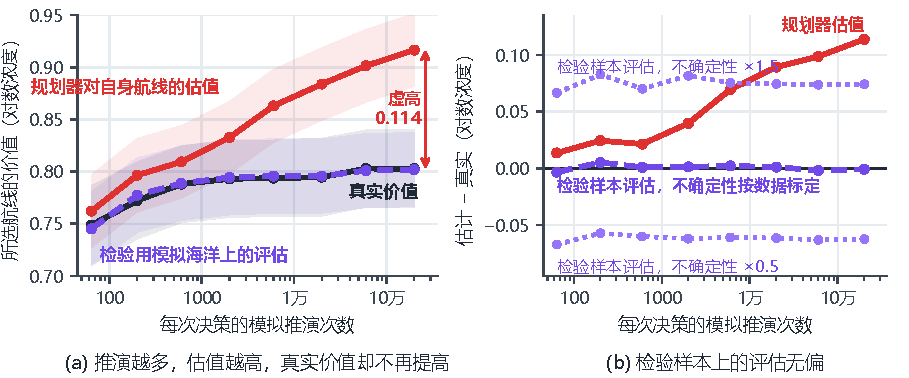
\includegraphics[width=\linewidth]{fig_curse}
\caption{前期东海赤潮巡测研究中的过度计算现象。(a) 所选航线的价值随每次决策推演次数的变化：规划器对自身航线的估值持续上升，真实价值与检验用模拟海洋上的评估约2000次后不再提高；(b) 估值减真实价值：规划器自身估值的高估随计算量增大，检验用模拟海洋上的评估保持无偏。多算让答案更精细，却不提供区分不同真实海洋的新信息。}
\label{fig:curse}
\end{figure}

第二种做法是把海流的不确定性纳入规划，但随机样本既难以估准关键方向上的效应，也不回答何时该去观测。集合规划在若干随机扰动流场（集合成员）上评估两侧航时，按集合平均选边或统计改变选边的成员比例\cite{wang2016path,subramani2018stochastic,kularatne2018forecast}。有限样本的平均受抽样误差左右；改变选边的成员比例只记录有多少成员改选，不度量改选后会多花多少时间，因而难以区分多花半小时与多花十几小时的任务\cite{benhaim2006infogap,marx2020predictive}。更重要的是，这类方法把不确定性当作固定输入，并不判断何时应停止计算、转而观测\cite{horvitz1987reasoning,russell1991right,lin2015metareasoning,elboher2023formal}。

第三种做法是主动观测，但为全场重构而采集的数据未必有助于选边。自适应采样引导航行器前往不确定性最高的海区，以降低全场估计误差\cite{srinivas2012gpucb,hollinger2014sampling,fossum2019}；然而，若某处误差对左右两侧的影响相同，测量它只是徒耗航时，若决定两侧快慢的切变远在数十千米之外，起点附近的测量也改变不了判断。序贯实验设计与模型判别理论指出，观测的价值在于区分要求不同行动的竞争假设\cite{chernoff1959sequential,box1967discrimination,garivier2016optimal,attia2018goal}。对选边而言，真正需要回答的问题因此是：与粗图同样相容的海流中，是否存在一个使另一侧更快的流场？它会让当前选择多花多少时间？

本文据此提出合理反例检验，其核心思想是：两侧难分高下有两种性质不同的原因，应分别交给计算与观测（图\ref{fig:overview}(d)）。若只是求解网格过粗、两侧航时差小于求解误差（数值歧义），加密计算即可看清粗图的本意；若粗图同时容许“左侧更快”与“右侧更快”的真实海流（环境歧义），算得再细也无法分辨，只能补充新信息。为区分二者，我们用多年再分析数据统计粗图的误差，划定与粗图相容的合理流场集合（合理集合），在其中搜索使另一侧更快的流场（合理反例），并计算坚持当前选择最多会多花的航时（最大后悔值）；最大后悔值超过阈值时，判定粗图对本次决定不可信，转而获取新信息。由于航时对流场的导数可以沿当前最快航线直接累加，这一检验只需数十次航线求解，适合在端侧运行。

本文的主要贡献有三点：
\begin{itemize}
    \item \textbf{区分数值歧义与环境歧义的决策判据。}据我们所知，本文首次在航行器航路决策中把“继续计算还是去观测”转化为一个可计算的问题——与粗图相容的海流中能否找到使另一侧更快的合理反例——并以最大后悔值衡量其代价：数值歧义交给计算，环境歧义交给观测。
    \item \textbf{由海洋大数据标定的合理集合与高效反例搜索。}合理集合的误差大小、空间相关长度与半径均由多年再分析误差标定；基于包络定理的梯度使每次迭代只需两次最短路求解，约71次求解即达到随机抽样2048次求解的选边效果。
    \item \textbf{跨海区与真实卫星图的系统验证。}在黑潮、湾流、阿古拉斯回流区以及改带卫星测高地转流图四种设置的逾两千个测试任务上，加算几乎不改变选错率，按最大后悔值排名前20\%的任务集中了53\%--71\%的额外航时；在粗图误差大的海区，被判定不可信后上浮取图使平均额外航时降低六成以上。
\end{itemize}

第\ref{sec:related}节回顾相关工作；第\ref{sec:problem}节建立问题模型并分析选边决策的难点；第\ref{sec:method}节给出合理反例检验方法；第\ref{sec:exp}节报告实验结果；第\ref{sec:innovation}节拆解本文的原创创新点与研究脉络；第\ref{sec:conclusion}节总结全文。
